\section{图同构与可达性：结构不依赖画法}
\label{sec:04-Discrete-Mathematics/03-Graph-Theory/10}

两个团队各自导出了一份服务依赖关系。节点 ID 一边是数据库主键，一边是服务名的哈希；布局工具也不同，一份画成放射状，一份画成分层。你要判断的是：这两份数据描述的是不是同一套依赖。

肉眼比对没有意义，两张图看着毫不相像。逐一试遍所有编号对应关系也不现实——六个节点就有 720 种对应，二十个节点超过 \(10^{18}\) 种。要回答这个问题，先得说清``同一张图''到底指什么。

\subsection{同构：把名字和位置一起忘掉}

图 \(G=(V,E)\) 与 \(H=(W,F)\) 同构，指存在双射 \(\phi:V\to W\)，使得

\[
\set{u,v}\in E
\quad\Longleftrightarrow\quad
\set{\phi(u),\phi(v)}\in F.
\]

双向箭头是要点：相邻的必须映成相邻，不相邻的也必须映成不相邻。只保证一个方向的映射会把边凭空添出来。

换成矩阵语言，重新编号就是用一个置换矩阵 \(P\)（每行每列恰好一个 1）同时置换行和列：

\[
B=P^{\trans}AP.
\]

行列必须一起换，因为邻接矩阵的行与列代表同一组顶点。只换行不换列，得到的矩阵不再是任何图的邻接矩阵。

\begin{center}
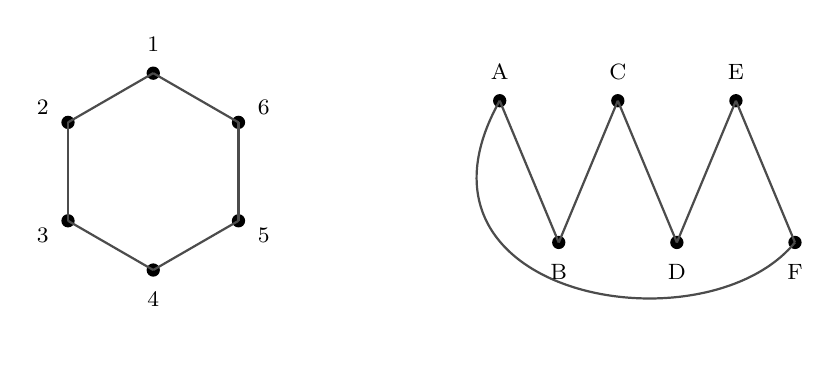
\begin{tikzpicture}[x=1cm,y=1cm,font=\small]
  \foreach \a/\n in {90/1,150/2,210/3,270/4,330/5,30/6}{
    \fill (\a:1.25) circle (2.4pt);
    \node[font=\footnotesize] at (\a:1.62) {\n};}
  \foreach \a/\b in {90/150,150/210,210/270,270/330,330/30,30/90}{
    \draw[thick,black!70] (\a:1.25) -- (\b:1.25);}

  \foreach \x/\n in {4.4/A,5.9/C,7.4/E}{
    \fill (\x,0.9) circle (2.4pt); \node[above,font=\footnotesize] at (\x,1.05) {\n};}
  \foreach \x/\n in {5.15/B,6.65/D,8.15/F}{
    \fill (\x,-0.9) circle (2.4pt); \node[below,font=\footnotesize] at (\x,-1.05) {\n};}
  \draw[thick,black!70] (4.4,0.9) -- (5.15,-0.9);
  \draw[thick,black!70] (5.15,-0.9) -- (5.9,0.9);
  \draw[thick,black!70] (5.9,0.9) -- (6.65,-0.9);
  \draw[thick,black!70] (6.65,-0.9) -- (7.4,0.9);
  \draw[thick,black!70] (7.4,0.9) -- (8.15,-0.9);
  \draw[thick,black!70] (8.15,-0.9) .. controls (7.0,-2.3) and (3.0,-1.6) .. (4.4,0.9);
\end{tikzpicture}

\emph{左边是六边形，右边像一条对接的折线，两幅画没有一处相似。可沿 \(A\to B\to C\to D\to E\to F\to A\) 走一圈就会发现右图也是一个六元环，对应 \(1\mapsto A,2\mapsto B,\dots,6\mapsto F\) 保住了全部邻接与不邻接。它们是同一张图。}
\end{center}

\subsection{不变量能否定，不能确认}

既然对应关系不好找，自然的想法是先算几个不随编号变化的量：顶点数、边数、度数的多重集、连通分量数、三角形个数、各长度的环数、邻接矩阵的特征值。这些量叫同构不变量。两张图只要有一项对不上，立刻判定不同构，开销很低。

麻烦在反方向。全部对上，什么也证明不了。

\begin{center}
\begin{tikzpicture}[x=1cm,y=1cm,font=\small]
  \foreach \a in {90,150,210,270,330,30}{\fill (\a:1.25) circle (2.4pt);}
  \foreach \a/\b in {90/150,150/210,210/270,270/330,330/30,30/90}{
    \draw[thick,black!70] (\a:1.25) -- (\b:1.25);}
  \node[font=\footnotesize] at (0,-1.95) {\(C_6\)：连通，无三角形};

  \begin{scope}[shift={(4.6,0)}]
    \foreach \a in {90,210,330}{\fill (\a:0.8) circle (2.4pt);}
    \foreach \a/\b in {90/210,210/330,330/90}{\draw[thick,black!70] (\a:0.8) -- (\b:0.8);}
  \end{scope}
  \begin{scope}[shift={(7.0,0)}]
    \foreach \a in {90,210,330}{\fill (\a:0.8) circle (2.4pt);}
    \foreach \a/\b in {90/210,210/330,330/90}{\draw[thick,black!70] (\a:0.8) -- (\b:0.8);}
  \end{scope}
  \node[font=\footnotesize] at (5.8,-1.95) {\(2C_3\)：两个分量，两个三角形};
\end{tikzpicture}

\emph{六个顶点、六条边、每点度数都是 2——度序列完全一致，两张图却显然不同构。三角形计数（0 对 2）能把它们分开，度序列不能。多加一项不变量只是把能分开的图多划走一批，从来不构成``它们相同''的证明。}
\end{center}

再加强也一样。特征值谱是相当精细的不变量，却也会失手：星形 \(K_{1,4}\) 与``一个四元环加一个孤立点''都有谱 \(\set{2,0,0,0,-2\,}\)，两张图连连通性都不同。这类同谱非同构的例子随着顶点数增加迅速变多。

这就是最典型的``必要条件不是充分条件''。不变量相同是同构的必要条件，把它当成充分条件用，就是在拿一个没有证明能力的检查冒充结论。区别在实践中很实在：不变量筛选适合做快速去重的第一道闸，把明显不同的图刷掉；剩下的候选还得真正找出对应关系才算数。

\subsection{它难，但难得不太一样}

图同构在复杂度地图上占着一个稀有的位置。至今没有已知的多项式时间算法，可它也不被认为是 NP 完全的——若它是，复杂度类的结构会出现许多人不相信的坍缩。Babai 在 2015 年给出拟多项式时间算法，这个结果本身就说明它不像哈密顿回路那样``硬''。实践中，nauty 之类的求解器在绝大多数真实图上飞快，只在精心构造的对抗实例上变慢。

上一节的对照可以在这里再叠一层：欧拉问题有简洁判据，哈密顿问题 NP 完全，图同构两头都不靠。``难''不是一个刻度，问题各自落在不同的位置上，工程判断要看落点而不是看直觉。

\subsection{颜色细化：一族不变量的上限}

有一种系统地生产不变量的办法。给每个顶点一个初始颜色（比如全部相同），然后反复更新：新颜色由``自己的旧颜色''加上``邻居旧颜色的多重集''决定，直到颜色划分不再变化。两张图若最终的颜色分布不同，必定不同构。这就是一维 Weisfeiler--Leman 检验，简称 1-WL。

它比度序列强得多，能分开的图多得多，可它照样只能否定。回头看上面那张图：\(C_6\) 和 \(2C_3\) 的每个顶点度数都是 2，邻居的颜色多重集从第一轮起就完全一致，往后每一轮都一致，永远分不开。给六边形和两个三角形贴颜色，1-WL 至死不改口。

这件事对做图数据的人有直接后果。消息传递式的图神经网络，每层做的正是``汇聚邻居表示再更新自己''，与颜色细化的结构一模一样。因此它的判别能力有一个上界：1-WL 分不开的两张图，标准的消息传递网络给出的图级表示也必然相同，无论加多少层、参数多大。若任务要求区分三角形数量不同而局部结构相同的图，得往模型里额外喂结构信息——子图计数、距离编码、随机特征，或者换用更高阶的架构。模型选型上的这个天花板，来源不是训练，而是本节这条``不变量只能否定''的老结论。

\subsection{可达性把一步邻接累积成任意长度}

同构关心``哪些外观差异无关''，可达性关心``哪些邻接关系会累积''。两者一起把结论从画法拉回邻接结构。

邻接矩阵的普通幂有明确含义：\((A^{k})_{ij}\) 等于从 \(i\) 到 \(j\) 长度为 \(k\) 的通道条数。若只关心能不能到，把非零元视为真，在 Boolean 代数里用``或''代替加法、``且''代替乘法，传递闭包就是

\[
R=I\lor A\lor A^{[2]}\lor\cdots\lor A^{[n-1]},
\]

其中 \(A^{[k]}\) 是 Boolean 意义下的幂。求和到 \(n-1\) 就停，是因为任何一条存在的通道都能把重复的环删掉，压成长度至多 \(n-1\) 的简单路径。

可达矩阵和最短路矩阵回答的不是同一个问题。前者只说能不能到，不记步数、不记代价、也不记路径条数。用普通整数幂再截成 0 和 1 能得到同样的存在信息，但要当心计数溢出——通道数增长得很快。算法上，Warshall 的动态规划、从每个顶点各做一次搜索、稀疏矩阵乘法各自适合不同的规模与稠密度。

无向图里可达关系把顶点划成连通分量。有向图里，若 \(u\) 能到 \(v\) 且 \(v\) 也能到 \(u\)，二者同属一个强连通分量。把每个强连通分量缩成一个点，得到的凝聚图必是有向无环图——否则环上那几个分量本来就该合并。网页链接、课程先修、软件依赖画出来都可能密密麻麻，可密集不等于互相可达；服务依赖里真正要紧的是有没有出现环，而不是图看着有多乱。

到这里，本单元的所有量都还只回答二值问题：连通不连通、同构不同构、画得下画不下。下一节问一个程度问题——一张连通的网络，究竟离断开还有多远。
